\documentclass[8pt]{beamer}
\usepackage[utf8]{inputenc}
\usepackage[danish]{babel}
\usepackage{amsmath}
\usepackage{ulem}
\usepackage{palatino}
\usepackage{graphicx}
\linespread{1.05}
\title{Team $\Delta$ - Pretested Integration}
\author{Alexander Uldall \and Andreas Frisch \and Esben Skaarup \and Ronni Lindsgaard}
\begin{document}
	\maketitle
	\section{The project}
		\begin{frame}{Project summary}
			\begin{itemize}
				\item We work for a company called Praqma who specialises in helping
				coorporations getting a control of their workflow and automate as much
				as possible.
				\item The goal of our project is to implement a pretested
				integration workflow for use with the mercurial SCM system with
				the Jenkins CI service.
			\end{itemize}
		\end{frame}
	
	\section{Sprint tasks}
		\begin{frame}{Formalia}
				\noindent
			\begin{description}
				\item[Sprint goal:] Make the plugin as generic as possible.
				\item[Theoretical sprint capacity:] $65~SP$
				\item[Velocity from last sprint:] $\frac{31~SP}{39~SP} \approx 0.79$
				\item[Actual sprint capacity] $65~SP \times 0.79 \approx  52 SP$
			\end{description}
		\end{frame}
		\begin{frame}{Sprint log - sprint \# 6}
			\begin{table}
				\center
				\begin{tabular}{|l|c|c|c|}
					\hline
					Task name & Priority & Estimate (SP) & Status \\
					\hline
					API: Post build handle & M & 3 & Resolved \\
					API: prep workspace & M & 2 & Resolved \\
					API: child class & M & 1 & Resolved \\
					API: success (Build success) & M & 2 & Resolved \\
					API Failure (Build failure) & M & 2 & Resolved \\
					Plugin interface class & M & 5 & Resolved \\
					Front end hax & M & 3 & Assigned \\
					Front end pretify & M & 3 & Assigned \\
					Prep workspace & M & 3 & Completed \\
					hg: handle build success & M & 2 & Resolved \\
					hg: handle build failure & M & 3 & Resolved? \\
					hg: popNextChild & M & 3 & Resolved \\
					hg: hasNexChild & M & 2 & Reopened \\
					Front-end magic & M & 2 & Not started \\
					hg: Define child & M & 3 & Invalid\\
					Assumptions in wiki/javadoc & M & 2 & Not started \\
					Plugin development in wiki/javadoc & M & 2 & Not started \\
					Getting started in wiki/jav doc & M & 3 & Not started \\
					Java docs & S & 3 & Not started \\
					Document architecture & S & 3 & Not started\\
					\hline
				\end{tabular}
			\end{table}
		\end{frame}
		\begin{frame}{Burnup chart}
			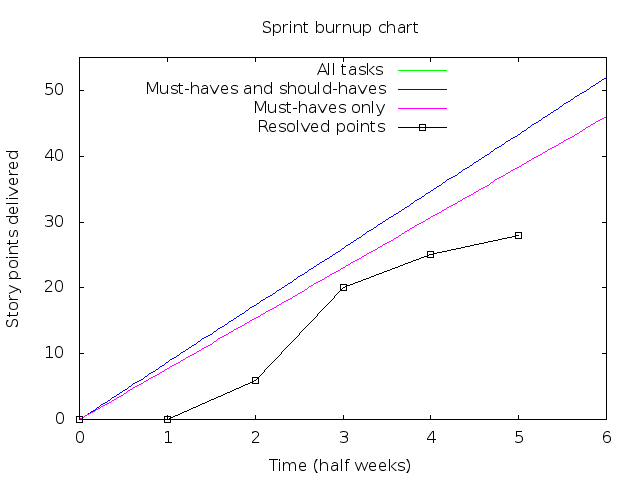
\includegraphics[width=\linewidth]{burnup.png}
		\end{frame}
		\begin{frame}{Demo}
			DEMO
		\end{frame}
\end{document}

